\documentclass{article}

\usepackage{graphicx}

\title{\textbf{Shreyas R}}
\date{\vspace{-5ex}}

\begin{document}
	\maketitle
	\hrulefill
	
	%Section 1
	\section{Introduction}
	\begin{flushleft}
		\textbf{Address} : 1552,16th Main Road,M C Layout
		Vijayanagar,Bangalore-560040
		\textbf{E-mail id} : rshreyas32@gmail.com
		\\\textbf{Contact Number} : 7411144517
		\begin{figure}[!ht]
			\begin{flushright}
				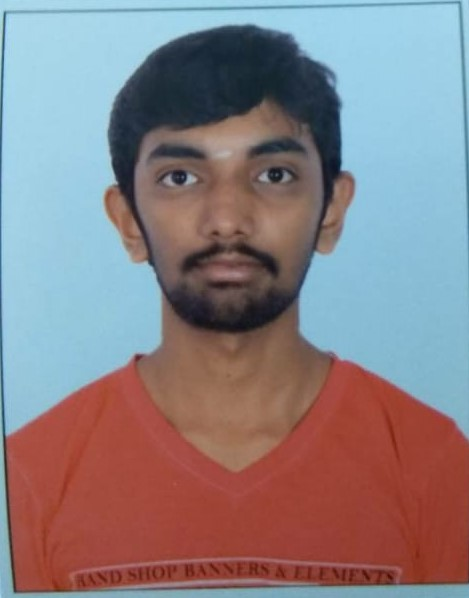
\includegraphics[width=20mm]{image.jpeg}
			\end{flushright}
		\end{figure}
	\end{flushleft}

	%Section 2
	\section{Carrer Objective}
	As a research enthusiast, I have never stopped exploring newer domains. An electronics and communication engineer,aiming to pursue a career in VLSI or embedded systems. Worked on various research projects while simultaneously managing academics.
	
	%Section 3
	\section{Education}
	\begin{table}[ht]
		\caption{Education}
		\centering
		\begin{tabular}{c c c c c}
			\hline\hline
			Course & Board & Institution & Year of passing & Aggregate \\[0.5ex]
			\hline
			BE 1st Year & PES University & PES University & 2018 & 9.23(CGPA) \\
			BE 3rd Semester & PES University & PES University & 2018 & 9.18(CGPA) \\
			12th & Karnataka PU Board & VVS Sardar Patel PU College  & 2017 & 94.83 \\
			10th & ICSE & Sri Vani Education Center & 2015 & 92.83 \\ 
			\hline
		\end{tabular}
		\label{table:nonlin}
	\end{table}

	%Section 4
	\section{Projects}
	\begin{enumerate}
		\item Audio-Video Transmission Using Li-fi.
		\item Data communication using ultrasonic sound.
		\item E-Yantra Robotics competition.
		\item Theoretical model for Collision Avoidance of debris for nano-satellites (Student Competition)
		\item Helmet and mask recognition in real-time using Tensorflow.
		\item Soccer robot.
		\item Density based traffic signal using 8051 microcontroller and IR sensors.
	\end{enumerate}

	%Section 5
	\section{Training and Internship}
	\begin{itemize}
		\item IOT workshop conducted by i3indya.
		\item Training at Visio Ai(Start-up), worked on helmet and mask recognition.
	\end{itemize}

	%Section 6
	\section{Research and Publications}
	\begin{enumerate}
		\item Applied for a conference for paper presentation on Audio and Video Transmission using Li-fi.
	\end{enumerate}

	%Section 7
	\section{Technical Skills}
	\begin{itemize}
		\item Programming Languages : Java , C , Python.
		\item Softwares Learnt : MATLAB, Eagle PCB design, Tensorflow.
		\item Worked on Arduino,Raspberry pi and 8051 Microcontroller.
	\end{itemize}

	%Section 8
	\section{Soft Skills}
	\begin{enumerate}
		\item Better teamwork and good co-ordination with people.
		\item Good at time management.
		\item Taking complete responsibility of the job assigned.
	\end{enumerate}

	%Section 9
	\section{Personal Information}
	\begin{itemize}
		\item Father’s Name : S N Ramachandra
		\item Mother’s Name : Anuradha S
		\item Sex: Male
		\item Date of Birth : 21-09-1999
		\item Nationality: Indian
	\end{itemize}

	%Section 10
	\section{Extra-Curricular Activities}
	\begin{itemize}
		\item Playing volleyball and table-tennis as recreational sports.
		\item Trekking is also one of my recreational activity.
		\item Yoga and meditation.
	\end{itemize}

	%Section 11
	\section{Co-Curricular Activities}
	\begin{enumerate}
		\item  Represented our school in inter-school cricket tournament and our department in college in inter-department sports.
		\item Won a few drama competitions in school.
	\end{enumerate}

	%Section 12
	\section{Declaration}
	I hereby, declare that all the information and facts provided is true to my best of knowledge.
	
	 
\end{document}
